\chapter{関連研究}
\label{chap:related_works}

関連研究、関連プロダクト、関連技術を示す。

\section{インスリンペン}

インスリンペンに関連したプロダクトは海外の企業が展開しているものがいくつかあり、摂取忘れや、管理に対する手法は様々である。
例としては、ペン型のインスリン注射器に装着する形のデバイス(以後、インスリンデバイスと呼ぶ)や、インスリンペンその物をスマートデバイス化したものがある。

\subsection{InPen}

InPenはアメリカのCompanion Medical社が開発したプロダクトであり、スマートデバイス化したインスリンペンと、スマートフォンアプリケーション(以下、「スマホアプリ」という。)がセットになっている。
インスリンペンはBluetoothを通してスマホアプリと連動させることができ、インスリンを摂取した時間とその量をログとして残し、可視化することができる。
また、タイマー式のリマインダで、例えば朝食前のインスリン服用であれば、6:00 - 9:00の間にインスリン摂取がログされていなかった場合はユーザーに通知を行うことが可能である。
スマホアプリは、DEXCOMという体内グルコース量を監視できるデバイスや、Bluetooth通信が可能なグルコース監視ツールとの連動も可能であり、これによりインスリン摂取量をガイドすることも可能としている。
しかしながら、こちらのプロダクトはインスリン摂取忘れを固定の時間設定で検知しているため、リアルタイム性に欠けており、当人の食事時間によっては忘れたことを気づくのが1時間後であったり、2時間後であったりするかもしれない。

\begin{figure}[htbp]
  \caption{InPenのペンとスマホプリ(文献\cite{inpen}より抜粋)}
  \label{fig:inpen_display}
  \begin{center}
    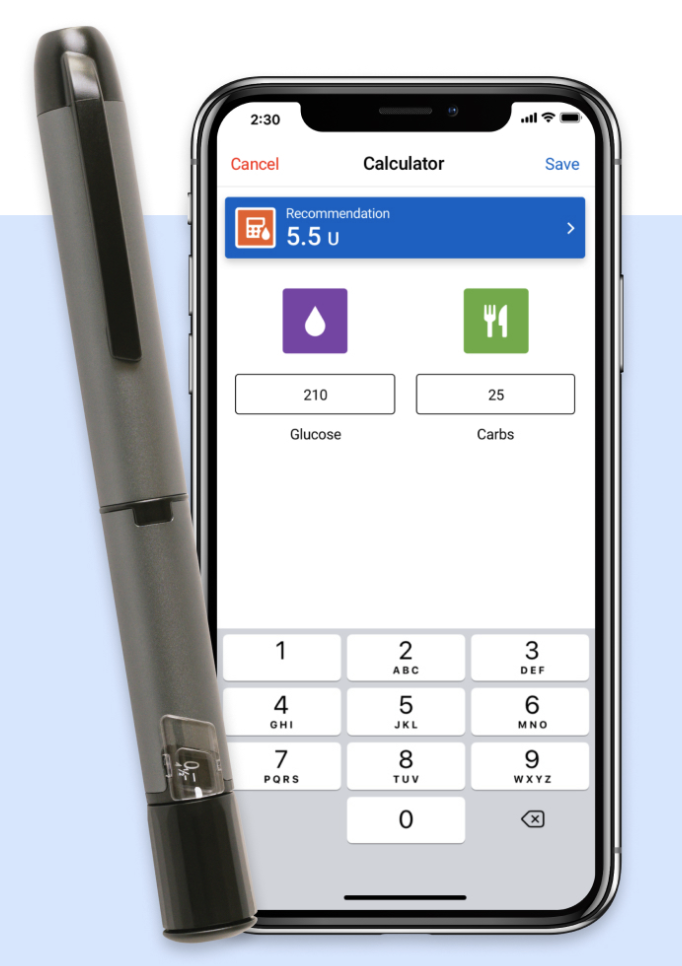
\includegraphics[bb=0 0 1000 500,width=10cm]{assets/inpen_display.png}
  \end{center}
\end{figure}

\subsection{insulCHECK}

insulCHECKはInnovation Zed社が開発したプロダクトであり、インスリンペンに装着するデバイスである。
このプロダクトは、インスリンが投与されたことを自動で検知し、その瞬間からタイムカウンターが経過時間を記録し始める。
患者は最終投与時間からどれくらい時間が経ったかを確認することで、直近でいつ自分がインスリンを摂取したか確認することができるので、
これによって、いつインスリンを打ったかどうか覚えておく必要がなくなり、2重投与などの事故の発生を防ぐことができる。
しかしながらこれは、患者自身が自分でペンを確認せねばならず、確認するという行為に至るまでのアクションの導線が存在しないため、
インスリンを打ち忘れていた場合には、患者自身が自ら気づく必要があり、受動的に打ち忘れを把握するための解決にはなっていない。

\begin{figure}[htbp]
  \caption{insulCHECKがインスリンペンに装着されている様子(文献\cite{insulcheck}より抜粋)}
  \label{fig:insulcheck_display}
  \begin{center}
    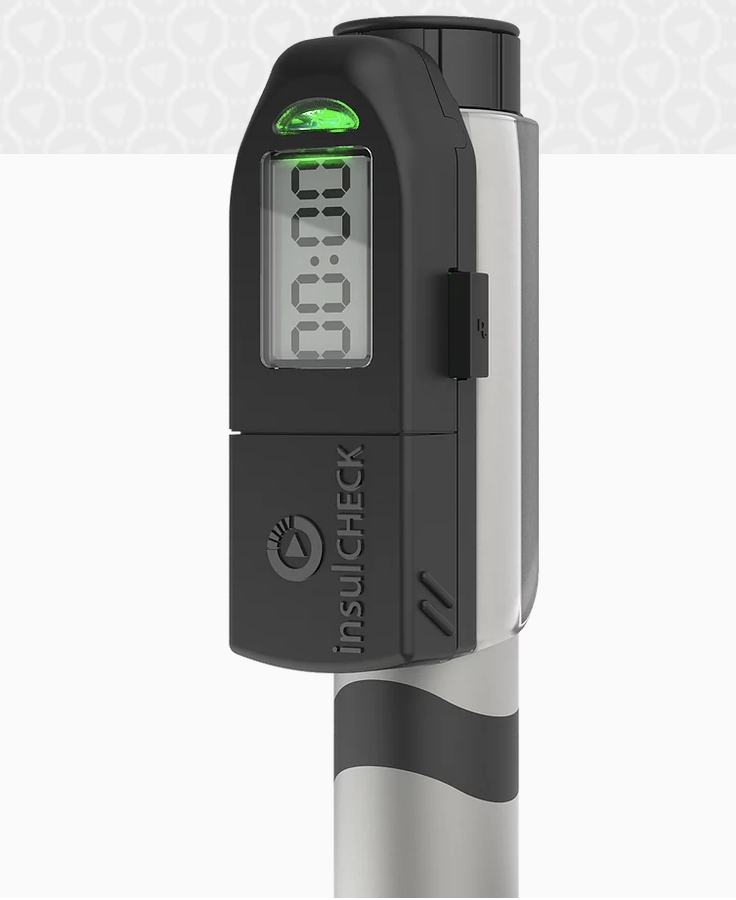
\includegraphics[bb=0 0 1000 500,width=10cm]{assets/insulcheck_display.png}
  \end{center}
\end{figure}

\subsection{Timesulin}

TimesulinはPatients Pending社が開発したプロダクトであり、インスリンペンのキャップの形をしたデバイスである。
これは、上記に挙げたinsulCHECKと同じく、タイムカウンターが実装されており、キャップが装着された瞬間から経過時間を記録し始める。
解決できる問題、また今回本研究で取り上げる課題に対する不足点はinsulCHECKを同様である。

\begin{figure}[htbp]
  \caption{Timesulinがインスリンペンに装着されている様子(文献\cite{timesulin}より抜粋)}
  \label{fig:timesulin_display}
  \begin{center}
    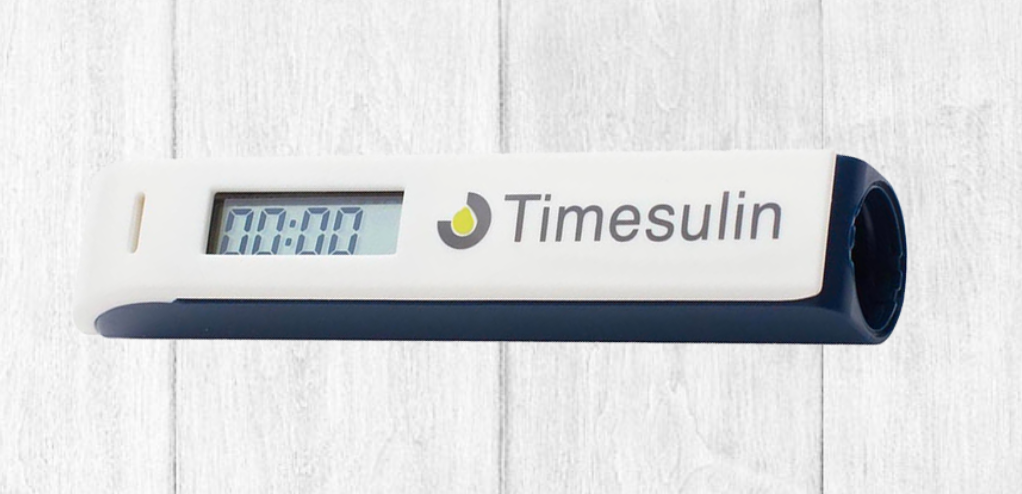
\includegraphics[bb=0 0 1000 500,width=10cm]{assets/timesulin_display.png}
  \end{center}
\end{figure}

\section{食事行動の検知}

肥満や摂食障害などは、心疾患や糖尿病など、生活習慣習慣病として人々の生活に大きな影響を与える。これらの治療には患者の食生活を把握し、管理する必要がある。
しかしながらこれらの監視、管理の多くは患者自身による曖昧な自主記録によるものが主流である。そして、これらの問題を解決するべく様々な研究がされており、
手法としてはウェアラブルセンサーデバイスを活用したもの \cite{wrist_motion_eating_detection} \cite{novel_wearable_device_monitor_ingestion} \cite{detect_eating_drinking_arm_gestures}
\cite{real_time_eating_wearable_device_eyeglass} \cite{eating_gestures_hidden_markov_models} \cite{detect_food_ingestion_chewing}や
カメラなどを活用して画像認識技術を利用したもの \cite{vb_fi_monitor_alzheimer} \cite{vb_fi_monitor_robot} \cite{vb_fi_monitor_mobile} 、そしてその両方を開け合わせたもの \cite{fi_monitor_camera_microphone} などがある。

ウェアラブルセンサー活用した手法でも、耳の下、下顎の付け根あたりに貼るセンサー(図\ref{fig:detect_food_ingestion_chewing}を参照)を活用したもの\cite{detect_food_ingestion_chewing}では、食事行動と、そうでない行動の分類精度が80.98\%だったとして、これを有用な手法であると述べている。
また、加速度センサーを内蔵した眼鏡型のデバイスと咀嚼を検知するためのこめかみに貼るセンサー(図\ref{fig:real_time_eating_wearable_device_eyeglass})を活用したも研究\cite{real_time_eating_wearable_device_eyeglass}では、食事シーンを歩いている時、休んでいる時、喋っている時などに分けてデータを学習させ、実験の結果、オフラインでの分類精度が93.15\%、
リアルタイムでのオンライン分類の精度が94.65\%だっとしており、リアルタイムでの食事行動の検知を正確に判定できると述べている。

さらに、画像認識技術を利用した食事行動検知では、図\ref{fig:vb_fi_monitor_alzheimer}のように食器の上に乗った食べ物も全てフレーム内におさめて、行動を認識させるもの\cite{vb_fi_monitor_alzheimer}や、
図\ref{fig:detect_chewing_jp}のように、顔の特徴量だけを利用して咀嚼を検知することで、被験者が食事をしているのか、ただ話しているだけなのかを判別する\cite{detect_chewing_jp}というものがある。
前者\cite{vb_fi_monitor_alzheimer}については、Haar-Cascade分類器を使用して実験を行ったところ、食事検知に対して、3.9フレーム毎秒で89\%の精度が出ており、さらに後者の研究\cite{detect_chewing_jp}においては、咀嚼の認識率が94\%であったと述べている。

これらの研究手法はどれも高精度で食事の検知を達成しているものの、顔の周辺に直接貼らなければならないセンサーや、眼鏡をかければならないものなど、実導入を考えるには現実的でない部分が見られる。
また、画像認識においても、正面から食事を撮影していなければならない点、使用する被験者は常に監視されているという不快感であったり、そのプライバシーを侵害しかねない可能性など、実導入に際しての障壁が高い。

本論文では、上記のような身体的な煩わしさ、映像で被験者を写すことで発生し得る障壁を極力なくし、それらの制約がない形での食事検知を目指す。

\begin{figure}[htbp]
  \caption{下顎のあたりにつける形のセンサー(文献\cite{detect_food_ingestion_chewing}より抜粋)}
  \label{fig:detect_food_ingestion_chewing}
  \begin{center}
    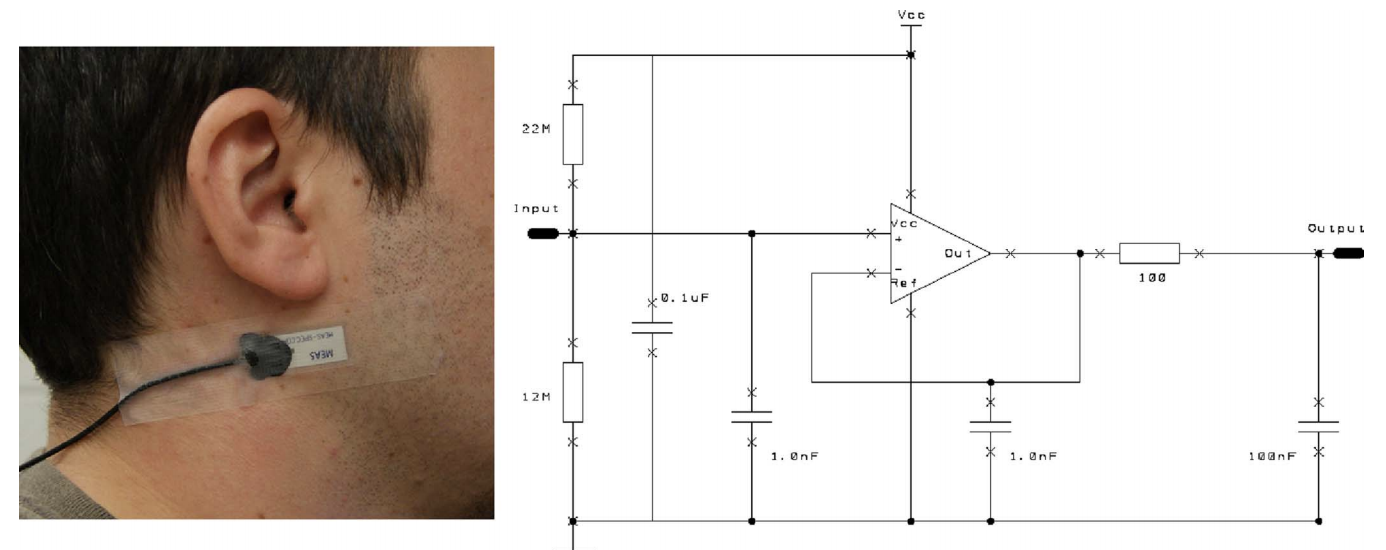
\includegraphics[bb=0 0 1000 500,width=10cm]{assets/fi_monitor_chewing.png}
  \end{center}
\end{figure}

\begin{figure}[htbp]
  \caption{眼鏡型のセンサーとこめかみに貼るセンサー(文献\cite{real_time_eating_wearable_device_eyeglass}より抜粋)}
  \label{fig:real_time_eating_wearable_device_eyeglass}
  \begin{center}
    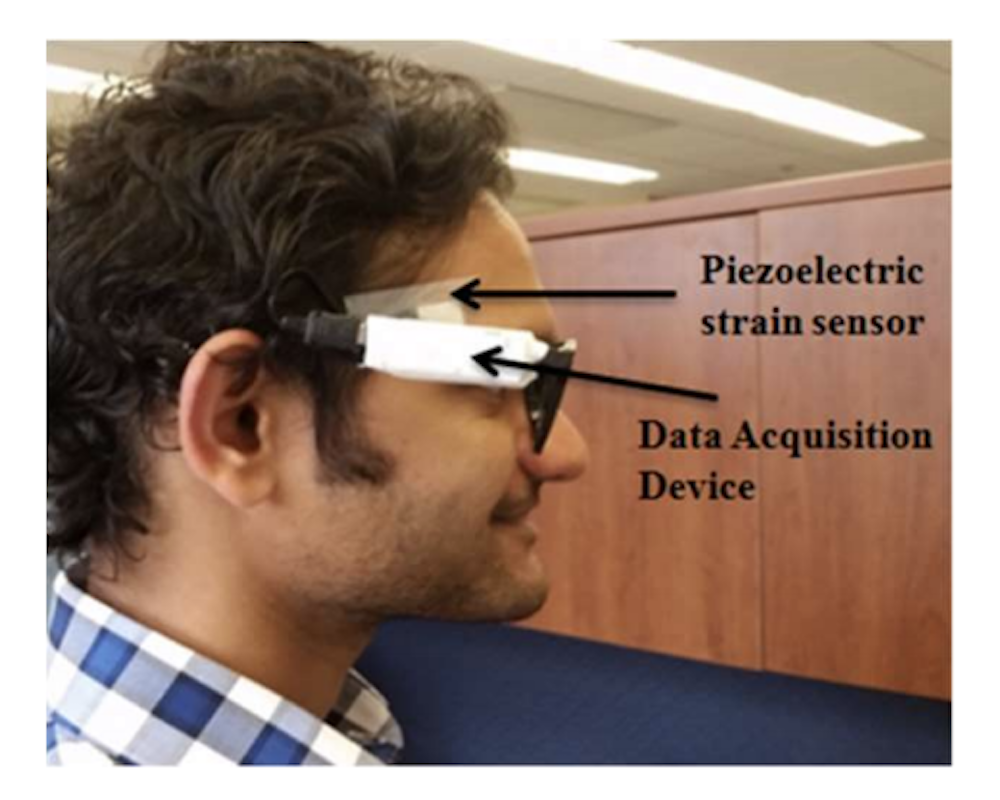
\includegraphics[bb=0 0 1000 500,width=10cm]{assets/fi_monitor_eyeglass.png}
  \end{center}
\end{figure}

\begin{figure}[htbp]
  \caption{画像認識を利用した食事行動検知(文献\cite{vb_fi_monitor_alzheimer}より抜粋)}
  \label{fig:vb_fi_monitor_alzheimer}
  \begin{center}
    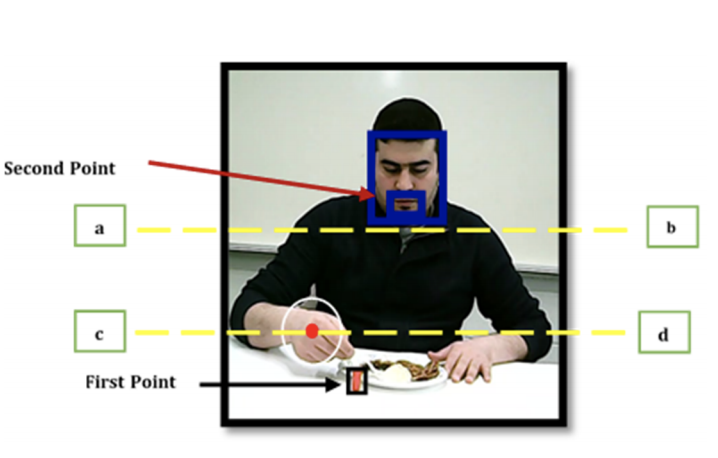
\includegraphics[bb=0 0 1000 500,width=10cm]{assets/vb_fi_monitor_alzheimer.png}
  \end{center}
\end{figure}

\begin{figure}[htbp]
  \caption{画像認識で顔の特徴量を利用した食事行動検知(文献\cite{detect_chewing_jp}より抜粋)}
  \label{fig:detect_chewing_jp}
  \begin{center}
    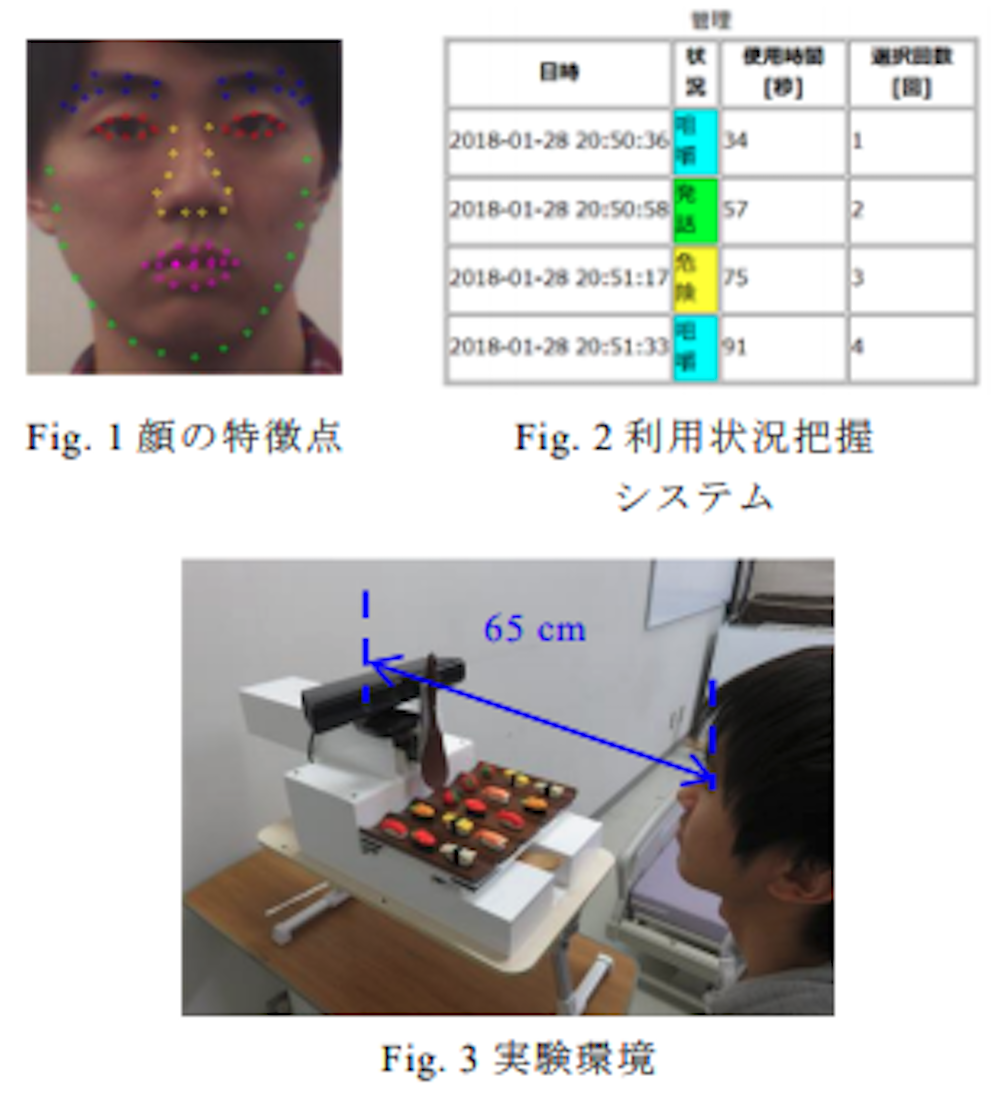
\includegraphics[bb=0 0 1000 400,width=10cm]{assets/detect_chewing_jp.png}
  \end{center}
\end{figure}

\section{関連技術}

本研究では、食事検知には食卓の振動を基に検知を試みるが、これには加速度センサーを用いている。
この節では、振動による人間の行動検知を行った研究を関連技術として示す。
文献\cite{floor_vibration_fall_detector}では、転倒が多く、それが死因にもなりうる高齢者の生活補助を目的に、床の振動を利用した自動転倒検知システムの提案を行っている。
この研究は、人間が転倒した際に床に伝わる衝撃や振動と、その他の歩く、タップするなどの活動による振動には大きく差があること、そして7kg程度の重さの物体が床に落ちる際の衝撃や振動は人間が点灯する際のそれとは大きく差があることを前提に
行われている。実装されたデバイス\ref{fig:floor_vibration_fall_detector}は、振動を検知するために圧電トランデューサーを内蔵しており、全体として1.5kgほどの重量である。
具体的な転倒の検知は、振動パターンの訓練の中で、閾値とその増幅値の設定を調整することで達成されたとしている。
この研究の実験・評価には、実験室試験場の中でダミーの人型人形を使用しており、結果としては、人間型ダミー人形の転倒で100\%検知、7kgほどの物体の落下で0\%検知となり、高精度での転倒検知が行われた。
% リノリウムコーティングがされたメザニンコンクリート床で距離にして約6m、スラブ打ちのコンクリート床で約4.5mの範囲内で転倒検知性能がそれぞれ、感度100\%(95\%の信頼区間(CI)94.87\%-100\%)と特異度100\%(95\%の信頼区間(CI)93.28\%-100\%)を達成したと述べている。
また、考察の中で、それまでのアプローチ存在していたウェアラブルデバイスのコンプライアンス的な問題や、画像認識によるプライバシー問題などの障壁を乗り越える手法として有効であると述べている。

\begin{figure}[htbp]
  \caption{圧電トランデューサーを見せるために横向きに置いた転倒検知デバイス(文献\cite{floor_vibration_fall_detector}より抜粋)}
  \label{fig:floor_vibration_fall_detector}
  \begin{center}
    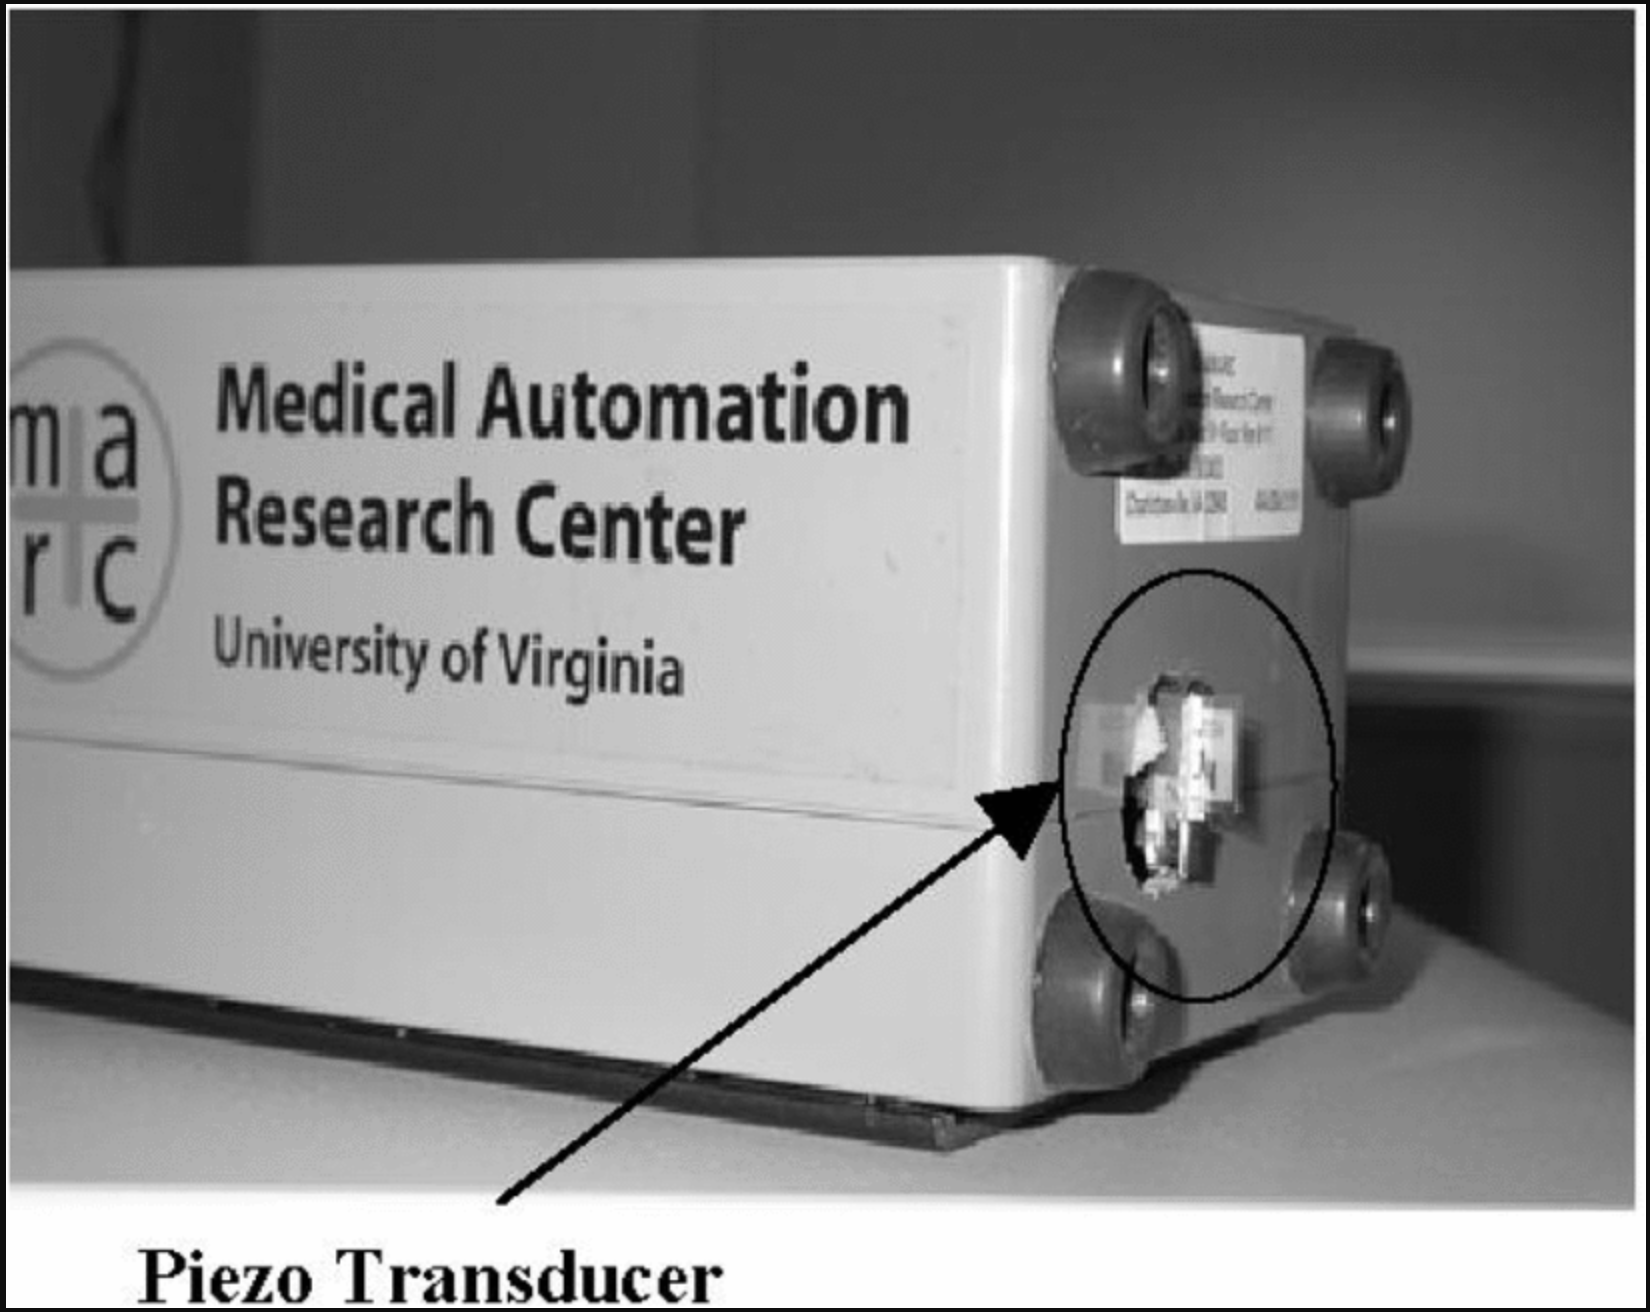
\includegraphics[bb=0 0 1000 800,width=10cm]{assets/floor_vibration_fall_detector.png}
  \end{center}
\end{figure}
